% !TEX TS-program = pdflatex
% !TEX encoding = UTF-8 Unicode

% This is a simple template for a LaTeX document using the "article" class.
% See "book", "report", "letter" for other types of document.

\documentclass[12pt]{article} % use larger type; default would be 10pt

\usepackage[utf8]{inputenc} % set input encoding (not needed with XeLaTeX)

%%%%\usepackage[document]{ragged2e} 

%%% Examples of Article customizations
% These packages are optional, depending on whether you want the features they provide.
% See the LaTeX Companion or other references for full information.

%%% PAGE DIMENSIONS
\usepackage{geometry} % to change the page dimensions
\geometry{letterpaper} % or letterpaper (US) or a5paper or....
\geometry{margin=1in} % for example, change the margins to 2 inches all round
% \geometry{landscape} % set up the page for landscape
%   read geometry.pdf for detailed page layout information

\usepackage{graphicx} % support the \includegraphics command and options
\graphicspath{
{figs/ipe/}
}
% \usepackage[parfill]{parskip} % Activate to begin paragraphs with an empty line rather than an indent

%%% PACKAGES
\usepackage{booktabs} % for much better looking tables
\usepackage{array} % for better arrays (eg matrices) in maths
\usepackage{paralist} % very flexible & customisable lists (eg. enumerate/itemize, etc.)
\usepackage{epstopdf}
\epstopdfsetup{suffix = {}}
\usepackage{siunitx}
\sisetup{unitsep = \cdot}
\usepackage{verbatim} % adds environment for commenting out blocks of text & for better verbatim
\usepackage{subfig} % make it possible to include more than one captioned figure/table in a single float
% These packages are all incorporated in the memoir class to one degree or another...

\usepackage{caption}        %Allows modification of captions
% \usepackage{indentfirst}    %Allows for indenting first paragraphs



\usepackage{hyperref}
\usepackage{todonotes}

%%% HEADERS & FOOTERS
\usepackage{fancyhdr} % This should be set AFTER setting up the page geometry
\pagestyle{fancy} % options: empty , plain , fancy
\renewcommand{\headrulewidth}{0pt} % customize the layout...
\lhead{}\chead{}\rhead{}
\lfoot{}\cfoot{\thepage}\rfoot{}

%%% SECTION TITLE APPEARANCE
\usepackage{sectsty}
\usepackage{tikz}
\usepackage[framemethod=TikZ]{mdframed}
\usepackage{enumerate}
\allsectionsfont{\sffamily\mdseries\upshape} % (See the fntguide.pdf for font help)
% (This matches ConTeXt defaults)

%%% ToC (table of contents) APPEARANCE
\usepackage[nottoc,notlof,notlot]{tocbibind} % Put the bibliography in the ToC
\usepackage[titles,subfigure]{tocloft} % Alter the style of the Table of Contents
\renewcommand{\cftsecfont}{\rmfamily\mdseries\upshape}
\renewcommand{\cftsecpagefont}{\rmfamily\mdseries\upshape} % No bold!

%%% END Article customizations

%%% The "real" document content comes below...

\title{Smart Control of 2-DOF Helicopter}
\author{Glenn Janiak \and Kenneth Vonckx \and \underline{Advisor}: Dr. Suruz Miah
}
%\date{} % Activate to display a given date or no date (if empty),
         % otherwise the current date is printed 
         
% \setlength{\parindent}{4em} % this should indent paragraphs

\begin{document}
\maketitle

\section{Project Description}
%\todo[inline]{} Previously used
%The aim of this project is to utilize machine learning techniques to control a team of helicopters.  Helicopters are very nonlinear and the dynamics complex, so control of them is challenging.  Convectional control techniques, such as (LQR) and LQG, are too simple to for this application.  Most research today based on simple control.  Additionally, this project will apply the concept of internet of things by providing a user interface for direct control via mobile devices. 

Helicopters are of a paramount importance as they are used in many civilian and military applications due to their ability for vertical take-off and landing.  To enable their use in such applications, intensive research has been conducted in the literature to date since helicopters involve complex nonlinear dynamics.  Most of the work on helicopter-based research requires dedicated computers for controlling their motion to specific configurations and resistant to turbulent conditions.  Such methods are expensive and time-consuming to develop.  Implementation of motion control techniques using cost-effective hardware is still a challenge.


In this project, we are proposing an algorithm for smart control of a team of two degree-of-freedom (2-DOF) helicopters using conventional motion control in cooperation with machine learning techniques where a user will be able to configure helicopters from any initial position.  Even though conventional techniques have been tested with simple platforms in the literature, the current project employs conventional motion control strategies in cooperation with machine learning technique (reinforcement learning, for instance) for a team of helicopters as well as introducing user control via mobile devices.  This project is expected to encourage research in this area as well as serve as an educational tool in teaching environments.   

%billions of dollars for
%aurdio (hobbies) platform for quanser


\section{System Architecture}
%Multiple helicopters will be controlled via embedded hardware interfacing devices which will receive input from a smart mobile device.  This general architecture is shown in \autoref{fig:ProblemStatementImage}.
%
\autoref{fig:highLevel} shows the high-level system architecture of the proposed project for control of a team of helicopters.  %
%
\begin{figure}
  \centering
  \begin{mdframed}[backgroundcolor=yellow!20, roundcorner=7pt,outerlinewidth=1.2pt,outerlinecolor=blue!50]
  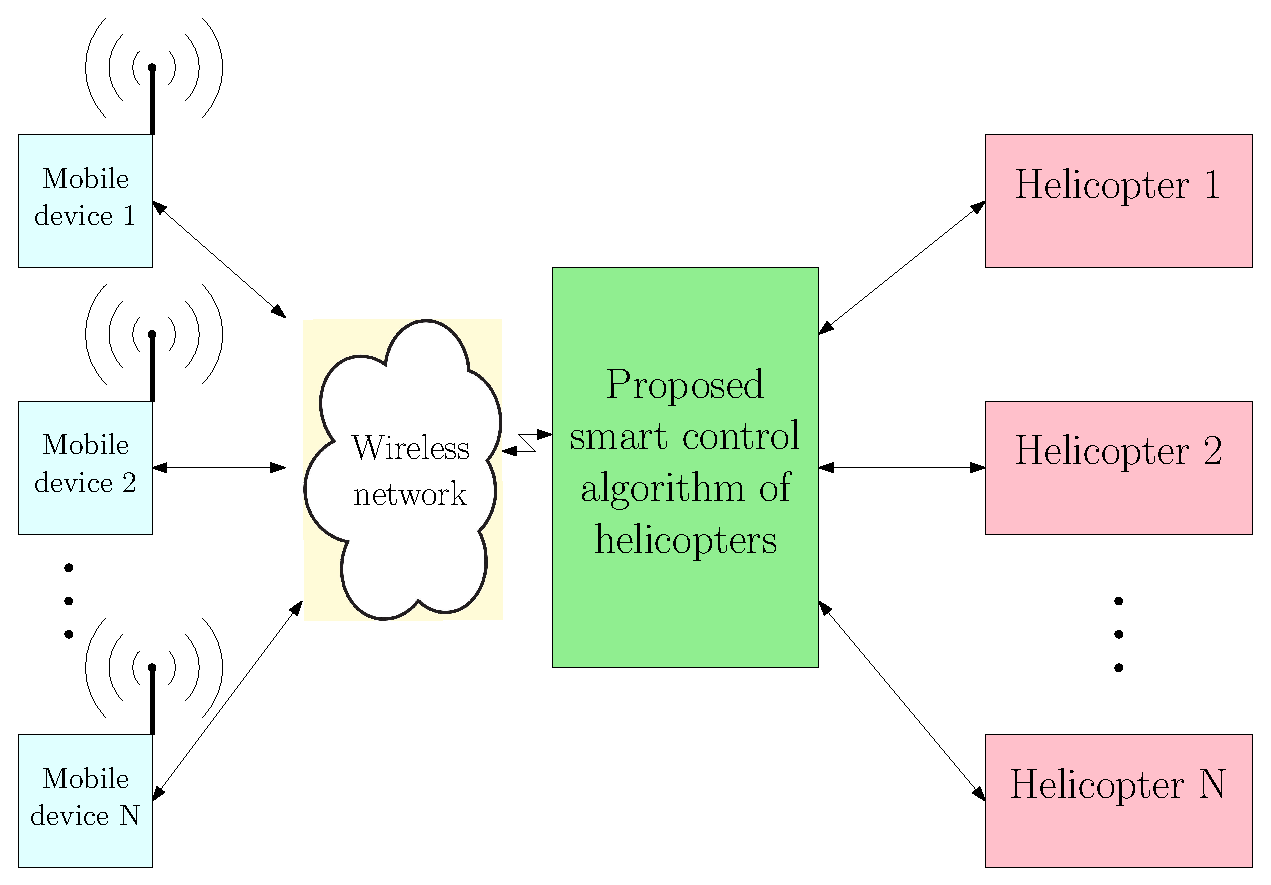
\includegraphics[scale=0.749]{figs/ipe/highLevel_yel_grn}
  \end{mdframed}
  \caption{General High-Level System Architecture}
  \label{fig:highLevel}
\end{figure}
%
As shown, mobile devices will serve as terminals for users to communicate with the helicopters.  Mobile devices can be used in a wider variety of locations over stationary and is desired by more people.  Information sent by the users will be transmitted through a wireless TCP/IP network.  Their inputs will interface with our proposed smart control algorithm and change the configuration of the helicopters.  In particular, we will be applying Linear Quadratic Regression (LQR), Linear Quadratic Gaussian (LQG), and a machine learning based algorithm for the control of these helicopters, Approximate Dynamic Programming (ADP).  

%Each of the helicopters we will be using have fixed bases as shown in \autoref{fig:QuanserAero} (courtesy of Quanser Inc.).

Each of the helicopters used will have fixed bases as shown in \autoref{fig:QuanserAero} (courtesy of Quanser Inc.).  

\begin{figure}
  \centering
  \captionsetup{justification=centering,margin=3cm}
  \includegraphics{figs/img/QuanserAero}
  \caption{Quanser Aero 2-DOF Helicopter \newline (\url{https://www.quanser.com/products/quanser-aero/})}
  \label{fig:QuanserAero}
\end{figure}
%
The tail of the helicopter has a motor that controls its yaw motion.  Similarly, the main rotor changes the pitch of the helicopter.  The directions in which the motors spin will be determined by the polarity of the applied voltages.  This will be regulated by our smart control algorithm.


\section{Modes of Operations}
%\label{sec:modesOfOperations}
We plan on allowing the user to control the helicopter using three modes of operation.  A short description of each mode is given below.

\begin{enumerate}[\textbf{Mode~\#}1:]
    \item Allows the user to control the helicopters to a given configuration. For example, setting the pitch to 45 degrees and the yaw to 90 degrees will move the helicopter that much from the initial configuration.
    \item Allows the user to choose a time varying input signal, so the helicopter will have a wave-like motion shifting from one configuration to another.  Examples include sine and square waves.
    \item Allows the user to control the algorithm that the user wishes to apply.  They will be able to choose from LQR, LQG, or ADP.
\end{enumerate}

\end{document}

%%% Local Variables:
%%% mode: latex
%%% TeX-master: t
%%% End:
